\documentclass[12pt,a4paper]{article}
\usepackage[a4paper,margin=1in]{geometry}
\usepackage{graphicx}
\usepackage{booktabs}
\usepackage{amsmath,amssymb}
\usepackage{float}
\usepackage{hyperref}
\usepackage{xcolor}
\usepackage{listings}
\usepackage{enumitem}
\usepackage{fancyhdr}
\usepackage{longtable}
\hypersetup{colorlinks=true,linkcolor=blue,urlcolor=blue}
\pagestyle{fancy}
\fancyhf{}
\lhead{ICS1512}
\rhead{Machine Learning Algorithms Laboratory}
\cfoot{\thepage}
\lstset{
language=Python,
basicstyle=\ttfamily\small,
numbers=left,
frame=single,
breaklines=true,
showstringspaces=false
}
\begin{document}
\begin{tabular}{|p{4cm}|p{11cm}|}
\hline
Experiment No. & 4\\ \hline
Experiment Title & Binary Classification using Logistic Regression and SVM\\ \hline
GitHub Repository & \url{https://github.com/Dharika-2006/ML-LAB-ASSIGMENTS} \\ \hline
Student Name & Dharika Shree K\\ \hline
Register Number & 3122247001014\\ \hline
Faculty & Dr. Poreddy Ajay Kumar Reddy \\ \hline
Submission Date & 02.08.26\\ \hline
\end{tabular}
\section{Objective}
To build and compare two binary classifiers -- Logistic Regression and Support Vector Machine (SVM) -- on the Spambase email dataset, tune their hyperparameters using GridSearchCV, and evaluate them using accuracy, precision, recall, F1-score, confusion matrices, ROC curves, and 5-fold cross-validation.

\section{Problem Statement}
\textbf{Problem:} Classify emails as spam or ham  using Logistic Regression and SVM, and compare which one works better on this dataset also testing SVM across four different kernels (linear, poly, rbf, sigmoid).

\textbf{Input:} The Spambase dataset , 57 numeric features describing word/character frequencies and capital-letter usage per email.

\textbf{Output:} Trained and tuned Logistic Regression and SVM models, kernel-wise SVM comparison, confusion matrices, ROC curves, cross-validation scores, and a final accuracy/precision/recall/F1 comparison between the two algorithms.

\section{Dataset Description}
\begin{longtable}{|p{6cm}|p{8cm}|}
\hline
Dataset Name & Spambase dataset\\ \hline
Dataset Source & Kaggle\\ \hline
Number of Samples & 4601\\ \hline
Number of Features & 57 \\ \hline
Number of Classes & 2 \\ \hline
Missing Values & None \\ \hline
Train-Test Split & 80\% training and 20\% testing\\ \hline
\end{longtable}

\section{Exploratory Data Analysis}
\begin{itemize}
\item Dataset overview
\item Statistical summary
\item Missing value analysis
\item Class distribution
\item Correlation matrix
\item Feature distribution
\end{itemize}

\subsection*{Figure: Class Distribution}
\begin{figure}[H]
\centering
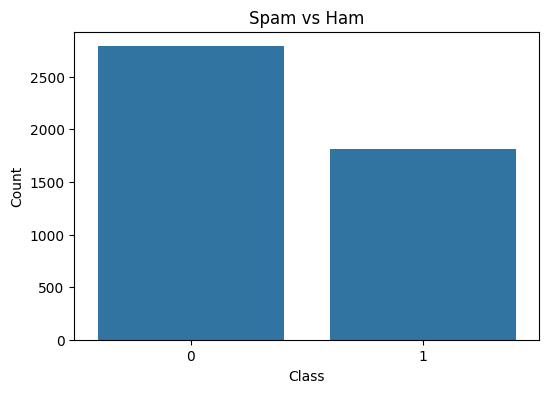
\includegraphics[width=0.6\linewidth]{cld1.png}
\caption{Spam vs Ham class counts}
\end{figure}
\textbf{Inference:}
About 60\% of the emails are ham and 40\% are spam (mean of the \texttt{class} column is 0.394), so it's not a perfectly balanced dataset but not extreme either. This is exactly why the train-test split was stratified -- to keep that same ratio in both splits -- and why we're looking at precision/recall/F1 and not just accuracy.


\subsection*{Figure: Statistical Summary}
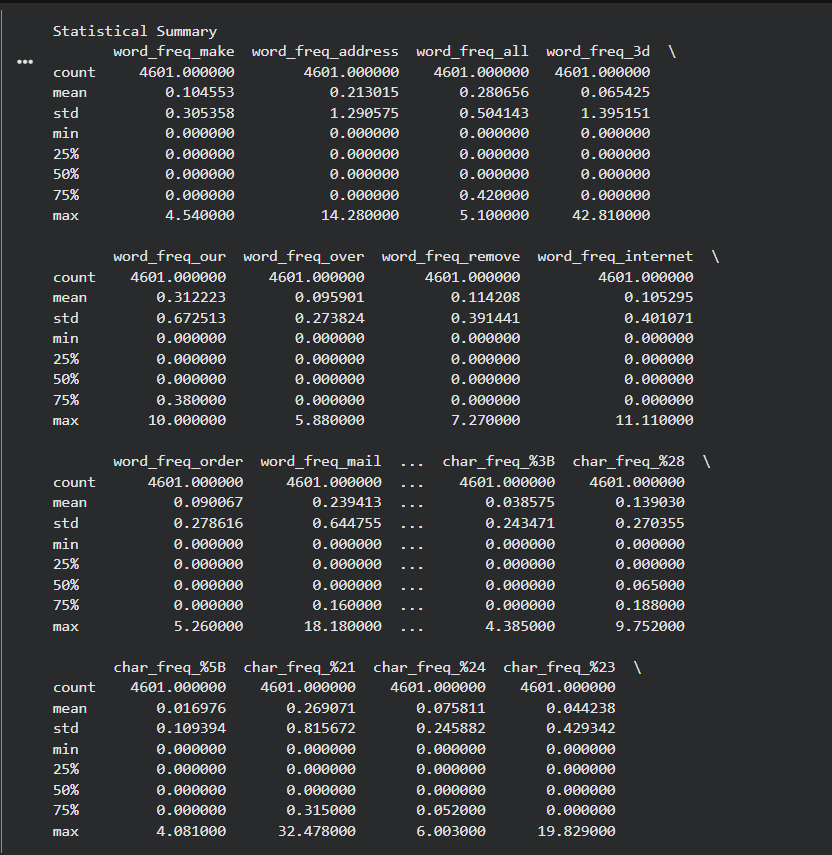
\includegraphics[width=0.5\linewidth]{summ.png}
\\
\textbf{Inference:}
The \texttt{describe()} output backs up what the histograms show -- for most features the 25th, 50th and 75th percentiles are all 0, meaning over half the emails have a frequency of 0 for that word, while the mean is pulled up by a handful of high-frequency outliers. No missing values anywhere, so no imputation was needed here (unlike the earlier experiments).

\subsection*{Figure: Correlation Matrix}
\begin{figure}[H]
\centering
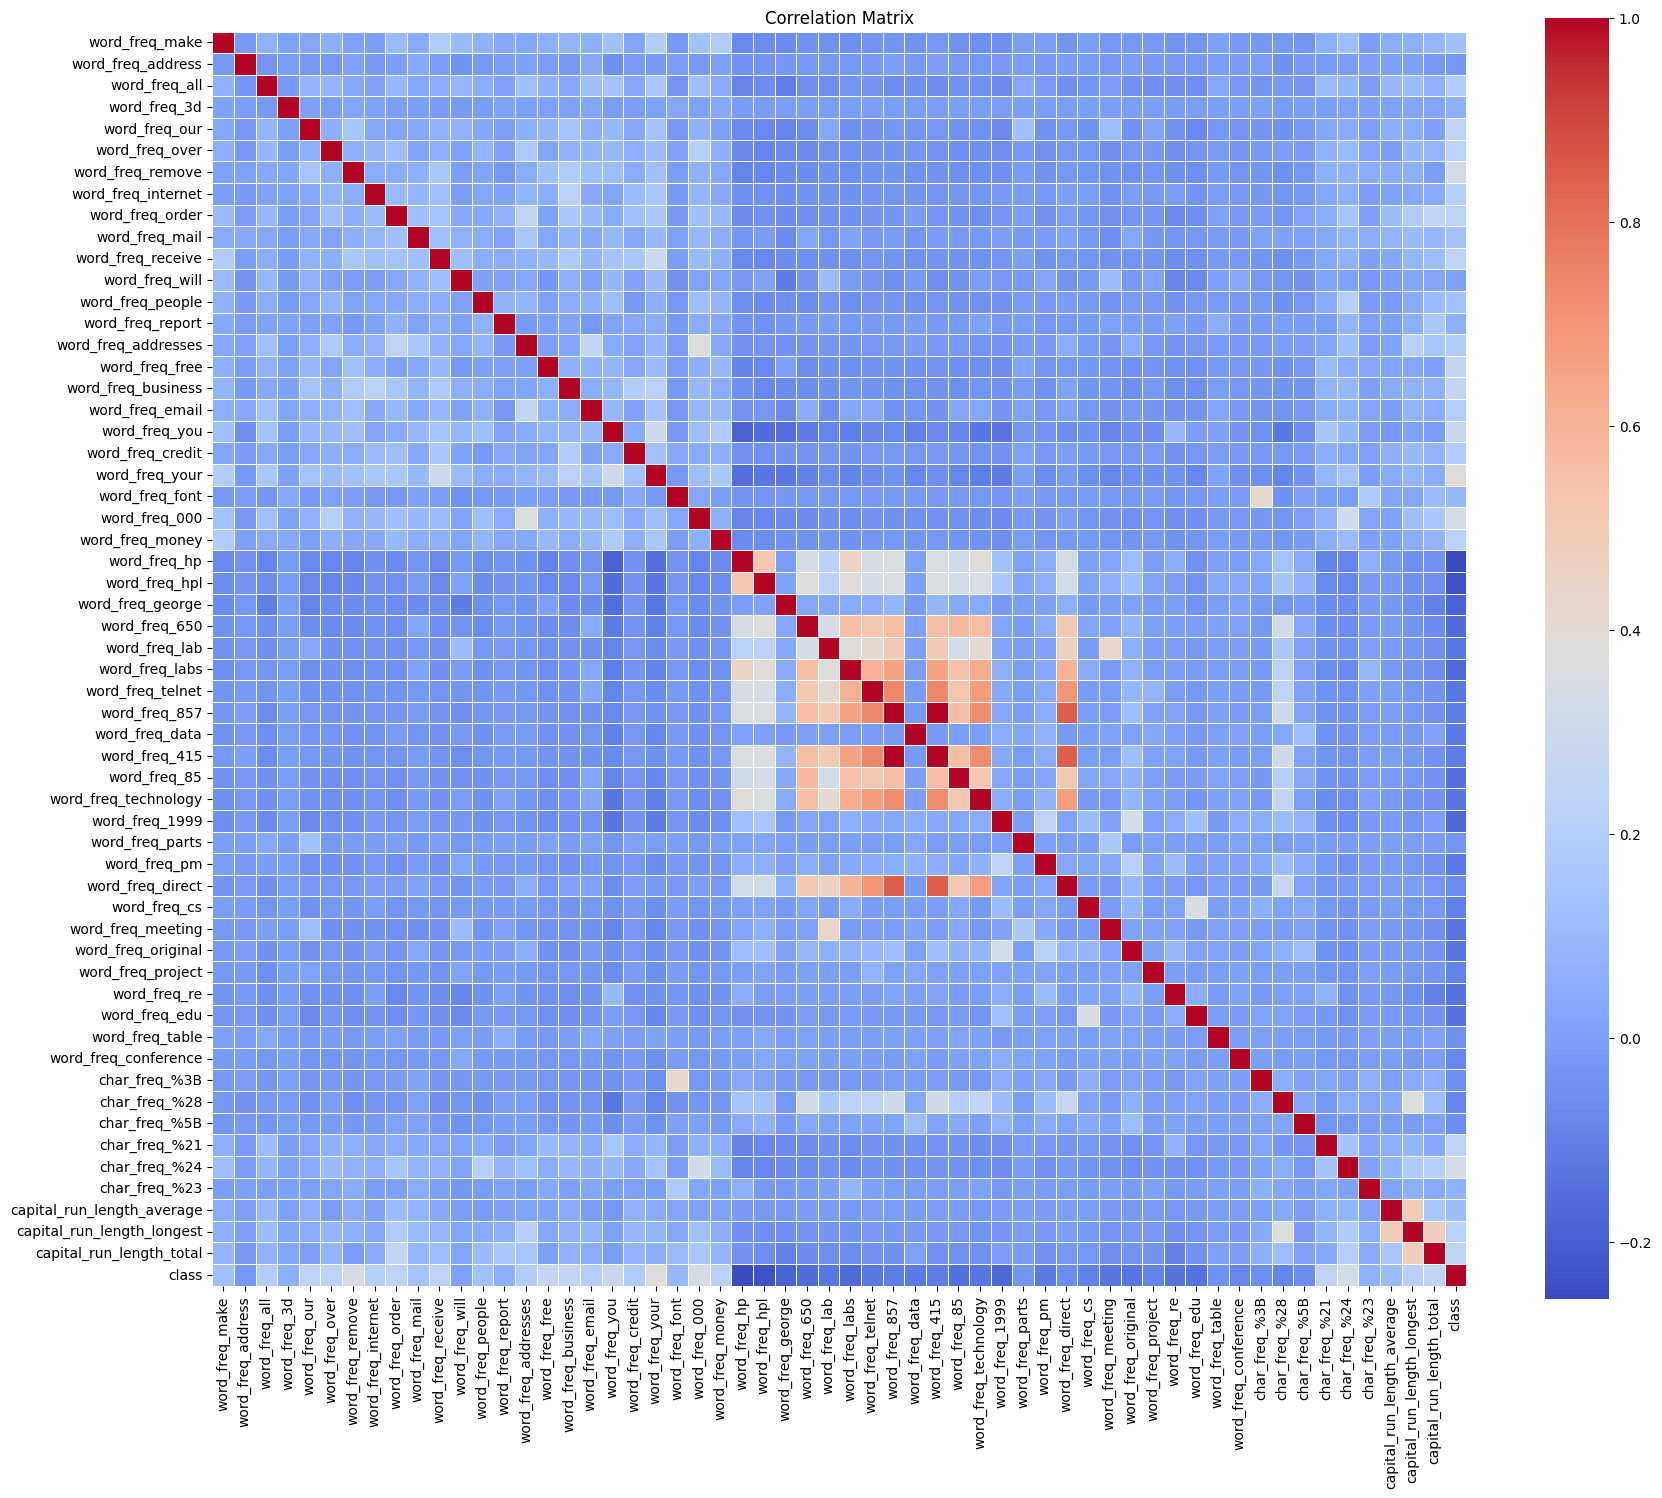
\includegraphics[width=1\linewidth]{corr.png}
\caption{Correlation heatmap of the 57 numeric features}
\end{figure}
\textbf{Inference:}
Most word-frequency features are only weakly correlated with each other, which works in favour of both models here -- Logistic Regression doesn't get too confused by multicollinearity, and SVM can find a clean separating boundary. A handful of related features (like the three capital-run-length stats, or spam-flavoured words like ``free'', ``money'', ``credit'') do move together and are the ones doing most of the heavy lifting in classification.

\section{Data Preprocessing}
\begin{itemize}
\item \textbf{Missing value handling:} Not needed -- the dataset had zero missing values.
\item \textbf{Encoding:} Not needed -- all 57 features are already numeric (word/character frequencies and capital-run-length stats).
\item \textbf{Feature scaling:} All features were standardized using \texttt{StandardScaler} (mean 0, unit variance) before training, since both Logistic Regression and SVM are distance/scale sensitive.
\item \textbf{Train-test split:} 80/20 split using \texttt{train\_test\_split} with \texttt{stratify=y} and \texttt{random\_state=42}, so the spam/ham ratio stays consistent in both sets.
\item \textbf{Feature engineering:} None -- the original 57 features were used as-is.
\end{itemize}

\section{Machine Learning Algorithm}
\subsection*{Logistic Regression}
\textbf{Working principle:} Models the log-odds of the positive class as a linear combination of the input features, then squashes it through the sigmoid function to get a probability.

\textbf{Mathematical formulation:}
\[
P(y=1\mid x) = \sigma(w^Tx + b) = \frac{1}{1+e^{-(w^Tx+b)}}, \qquad
\min_{w,b}\ -\sum_i \big[y_i\log \hat{y}_i + (1-y_i)\log(1-\hat{y}_i)\big] + \lambda \, \Omega(w)
\]
where $\Omega(w)$ is the L1 or L2 penalty term (tuned via the \texttt{penalty} hyperparameter in this experiment).

\textbf{Advantages:} Fast, interpretable coefficients, works well when classes are roughly linearly separable, cheap to train (0.04s in this experiment).

\textbf{Limitations:} Struggles with non-linear decision boundaries, sensitive to outliers and unscaled features.

\subsection*{Support Vector Machine (SVM)}
\textbf{Working principle:} Finds the hyperplane that maximizes the margin between the two classes; the kernel trick lets it draw non-linear boundaries by implicitly mapping data into a higher-dimensional space.

\textbf{Mathematical formulation:}
\[
\min_{w,b}\ \tfrac{1}{2}\|w\|^2 + C\sum_i \xi_i \quad \text{s.t.}\ y_i(w^T\phi(x_i)+b) \ge 1-\xi_i
\]
Kernels tested: linear $K(x,x')=x^Tx'$, polynomial, RBF $K(x,x')=e^{-\gamma\|x-x'\|^2}$, and sigmoid.

\textbf{Advantages:} Handles non-linear boundaries well via kernels, generally robust to overfitting when $C$ is tuned properly, gave the best precision of all models tested (0.928 with the tuned RBF kernel).

\textbf{Limitations:} Slower to train than Logistic Regression (2s for the linear kernel vs.\ 0.04s for Logistic Regression), more hyperparameters to tune ($C$, $\gamma$, kernel choice), and the polynomial kernel here badly underperformed (recall of just 0.46), showing how much kernel choice matters.

\section{Experimental Setup}
\begin{tabular}{ll}
\toprule
Python Version & 3 (exact version not captured; run on Google Colab's Python 3 runtime)\\
Scikit-Learn Version & As installed in the Colab environment (verify with \texttt{sklearn.\_\_version\_\_})\\
IDE & Google Colaboratory (Jupyter-based notebook)\\
Operating System & Linux (Google Colab backend)\\
Hardware & Google Colab-provided CPU runtime\\
\bottomrule
\end{tabular}

\section{Hyperparameter Selection}
\begin{tabular}{ll}
\toprule
Parameter & Value\\
\midrule
Train-Test Split & 80:20, stratified, \texttt{random\_state=42}\\
Cross-Validation & 5-fold, scoring = accuracy\\
Logistic Regression -- search space & $penalty\in\{l1,l2\}$, $C\in\{0.01,0.1,1,10,100\}$, $solver\in\{liblinear,saga\}$\\
Logistic Regression -- best params & $C=1$, $penalty=l1$, $solver=saga$ (Best CV Accuracy = 0.9239)\\
SVM -- search space & $kernel\in\{linear,rbf\}$, $C\in\{1,10\}$, $gamma=scale$\\
SVM -- best params & $C=1$, $gamma=scale$, $kernel=rbf$ (Best CV Accuracy = 0.9340)\\
\bottomrule
\end{tabular}

\section{Results}
\begin{longtable}{lcccc}
\toprule
Model & Accuracy & Precision & Recall & F1-score\\
\midrule
Logistic Regression (tuned) & 0.9294 & 0.9209 & 0.8981 & 0.9093\\
SVM (tuned, RBF kernel) & 0.9273 & 0.9277 & 0.8843 & 0.9055\\
\bottomrule
\end{longtable}
\noindent Logistic Regression edges out SVM slightly on accuracy, recall and F1, while tuned SVM has a marginally better precision. Honestly, the two models land within about 0.2\% of each other on accuracy -- close enough that either would be a reasonable choice here.

\section{Result Visualization}
Include all graphs generated during the experiment.

\subsection*{1. Correlation Matrix}
See Section 4 -- weak correlations between most features, a few standout groups (capital-run-length stats, spam-flavoured words) driving most of the signal.

\subsection*{2. Class Distribution}
See Section 4 -- roughly 60/40 ham-to-spam split.

\subsection*{3. Confusion Matrix}
\begin{figure}[H]
\centering

\includegraphics[width=0.55\linewidth]{conf1.png}
\caption{Confusion Matrix -- Logistic Regression}
\end{figure}
\begin{figure}[H]
\centering

\includegraphics[width=0.55\linewidth]{conf2.png}
\caption{Confusion Matrix -- SVM (RBF kernel)}
\end{figure}
\textbf{Inference:}
Both models make more false-negative errors (spam missed as ham) than false-positive ones, which lines up with recall (0.898 for LR, 0.884 for SVM) being a touch lower than precision for both. Logistic Regression catches slightly more spam overall, while SVM is a bit more cautious before calling something spam -- which is why its precision is marginally higher.

\subsection*{4. ROC Curve}
\begin{figure}[H]
\centering
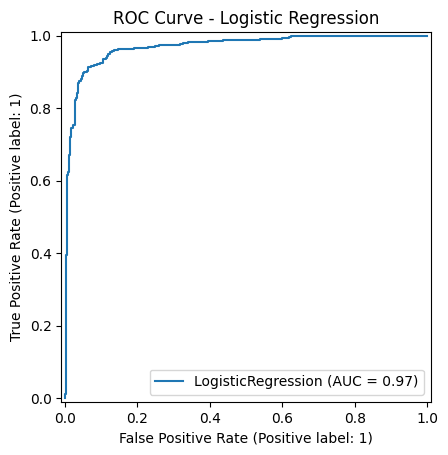
\includegraphics[width=0.55\linewidth]{logcurve.png}
\caption{ROC Curve -- Logistic Regression}
\end{figure}
\begin{figure}[H]
\centering
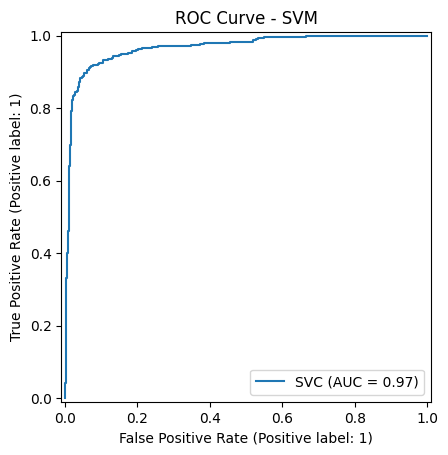
\includegraphics[width=0.55\linewidth]{curve2.png}
\caption{ROC Curve -- SVM}
\end{figure}
\textbf{Inference:}
Both ROC curves hug the top-left corner pretty tightly, which fits with both models scoring above 0.92 accuracy. There's no dramatic separation between the two curves -- consistent with how close their F1-scores are overall.

\subsection*{5. Precision-Recall Curve}
Not generated separately in the notebook (ROC curves were used instead), but the precision/recall numbers already reported tell the same story: SVM trades a bit of recall for precision compared to Logistic Regression.

\subsection*{6. SVM Kernel Comparison}
\begin{figure}[H]
\centering
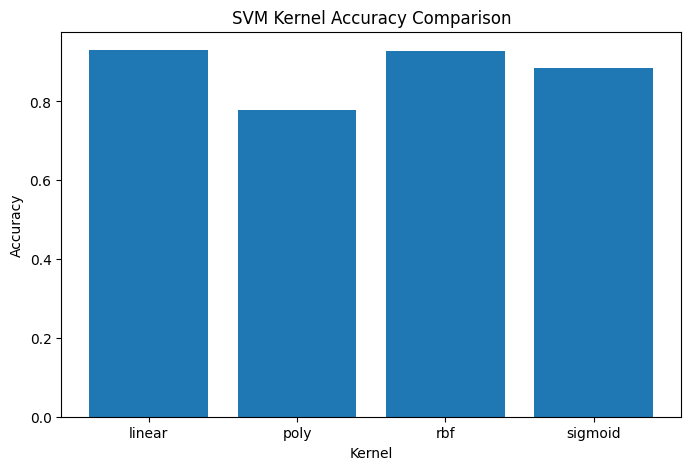
\includegraphics[width=0.7\linewidth]{comp.png}
\caption{Accuracy across the four SVM kernels}
\end{figure}
\textbf{Inference:}
Linear (0.9305) and RBF (0.9273) kernels are clearly the strongest performers, sigmoid trails behind at 0.884, and poly is by far the worst (0.780 accuracy, and only 0.46 recall) -- it's basically missing more than half the spam emails. This shows the data is close to linearly separable, so the extra flexibility of poly/sigmoid kernels doesn't help and, if anything, hurts here.

\subsection*{7. Learning Curve}
Not generated for this experiment (GridSearchCV was used instead of learning curves for tuning diagnostics).

\subsection*{8. Feature Importance}
Not explicitly plotted, but Logistic Regression's coefficients (via the L1 penalty selected by GridSearchCV) would naturally zero out less useful features, and the correlation matrix already hints that capital-letter usage and spam-associated words are the most predictive features.

\section{Discussion}
Both models did well here -- north of 92\% accuracy each -- which isn't too surprising given Spambase is a fairly clean, well-studied dataset once scaled properly. Logistic Regression came out very slightly ahead on accuracy/recall/F1, and it's also way cheaper to train (milliseconds vs.\ seconds for SVM), so honestly it's the more practical pick if training time or interpretability matters. The one thing worth flagging: GridSearchCV for Logistic Regression took 581 seconds (almost 10 minutes!) because of the \texttt{saga} solver combined with L1 -- that's a big cost for landing on basically the same performance as the untuned baseline. On the SVM side, kernel choice mattered a lot more than expected: poly kernel completely fell apart on recall (0.46), showing that not every kernel suits every dataset, and rbf/linear were clearly the better bets. Cross-validation results (SVM averaging 0.923, Logistic Regression 0.911 across 5 folds) also back up that both models are fairly stable, though fold 5 dipped noticeably for both, which is probably just a harder split of the data. If I were pushing this further, I'd try feature selection to cut down the 57 features, maybe try a Random Forest for comparison, and also look at why fold 5 underperformed.

\section{Conclusion}
This experiment compared Logistic Regression and SVM (across four kernels) for spam classification on the Spambase dataset. After hyperparameter tuning, Logistic Regression (C=1, L1 penalty, saga solver) slightly outperformed the best SVM (RBF kernel, C=1) on accuracy, recall and F1, while SVM edged ahead on precision. Given how close the two are and how much faster Logistic Regression is to train, it comes across as the more practical choice for this dataset -- though SVM with the right kernel (linear or RBF, definitely not poly) is a solid alternative. Overall, the experiment reinforced that simpler, well-regularized linear models can hold their own against more complex kernel methods when the underlying data is close to linearly separable, as Spambase turned out to be.

\section{References}
\begin{enumerate}
\item Scikit-learn developers,Logistic Regression,scikit-learn documentation: \url{https://scikit-learn.org/stable/modules/linear_model.html#logistic-regression}
\item Scikit-learn developers,Support Vector Machines,scikit-learn documentation: \url{https://scikit-learn.org/stable/modules/svm.html}
\item Kaggle,Spambase dataset,Kaggle Datasets: \url{https://www.kaggle.com/datasets}
\end{enumerate}
\end{document}